\chapter{Đánh giá}

\section{Đánh giá chất lượng đầu ra của lộ trình học đề xuất bởi LLM}

\subsection{Phương án đánh giá}
Trong bối cảnh đánh giá hệ thống sinh lộ trình học tập, có hai hướng tiếp cận để đánh giá \cite{zhang2020new}:
\begin{itemize}
    \item \textbf{Online evaluation} là phương pháp sử dụng phản hồi thực tế từ người dùng hoặc chuyên gia để đánh giá chất lượng đầu ra. Phương pháp này có độ tin cậy cao và phản ánh đúng nhu cầu thực tế, tuy nhiên yêu cầu thời gian, chi phí lớn và khó mở rộng trong giai đoạn phát triển ban đầu.
    \item \textbf{Offline evaluation} là phương pháp sử dụng mô hình hoặc thuật toán đánh giá tự động để đánh giá đầu ra mà không cần tương tác với người dùng, về dữ liệu, những dữ liệu cũ quan sát được trong quá khứ có thể được sử dụng cho Offline evaluation.
\end{itemize}
Trong báo cáo này, nhóm lựa chọn phương pháp \textbf{offline evaluation kết hợp với GEval} – một framework đánh giá tự động sử dụng mô hình ngôn ngữ lớn (LLM) làm giám khảo (LLM-as-a-Judge)\cite{liu2023gevalnlgevaluationusing}. GEval cung cấp một framework linh hoạt để định nghĩa các tiêu chí đánh giá tuỳ chỉnh, kết hợp với chuỗi suy luận (Chain-of-Thought) để hướng dẫn mô hình đưa ra lập luận có cơ sở. GEval có những điểm phù hợp để được chọn làm metric cho  phần đánh giá này vì:
\begin{itemize}
    \item Không cần dữ liệu tham chiếu cố định (reference output).
    \item Thực hiện đánh giá nhanh, lặp đi lặp lại và có thể tự động hóa được với nhiều tập dữ liệu khác nhau.
    \item Dễ mở rộng cho nhiều tiêu chí khác nhau như chất lượng giải thích, tính logic, mức độ phù hợp mục tiêu,...
    \item Có thể sử dụng với nhiều mô hình đánh giá khác nhau như: gpt-4o, gpt-4o-mini, llama-3.2,...
\end{itemize}

\subsection{Xây dựng các metrics}
Dựa trên metric GEval được đề cập ở trên, các metric sau được lựa chọn để đánh giá sơ bộ đầu ra của hệ thống:
\begin{itemize}
    \item \textbf{Goal Alignment (Goal)}: Lộ trình có bám sát mục tiêu học tập không?
    \item \textbf{Explanation Quality (Expl.)}: Chất lượng và độ rõ ràng của giải thích lý do trong từng bài học được đề xuất.
    \item \textbf{Ordering Logic (Order)}: Trình tự các bài học có hợp lý và phát triển kiến thức tuyến tính không?
    \item \textbf{Module Appropriateness (Mod. App.)}: Các module có phù hợp với nội dung bài học và mục tiêu không?
\end{itemize}

Metric GEval được sử dụng làm nền tảng để tự động hóa quá trình đánh giá, cụ thể:
\begin{itemize}
    \item Xây dựng tiêu chí đánh giá cho từng metrics, tương tự như việc xây dựng một rubrics để chấm điểm và các tiêu chí này phải càng cụ thể, giống như con người thực hiện việc đánh giá cũng cần rubrics.
    \item Model đánh giá (evaluator) được yêu cầu cho điểm (score) và giải thích (reasoning).
    \item Các trọng số được áp dụng cho từng metric để tính tổng điểm cuối cùng (final score).
\end{itemize}
Chi tiết về các metrics được định nghĩa cho phần đánh giá, người đọc có thể xem chi tiết trong phần code ở \href{https://github.com/dpnam2112/codemate-backend/blob/main/tests/metrics.py}{đây}\footnote{\url{https://github.com/dpnam2112/codemate-backend/blob/main/tests/metrics.py}}.

\subsection{Thiết kế quy trình đánh giá}
Do hạn chế về tài nguyên cũng như một số ràng buộc từ các nhà cung cấp dịch vụ để sử dụng mô hình của OpenAI, Google,... nên hiện tại, nhóm chỉ có thể triển khai việc đánh giá với phương pháp này ở mức cơ bản và về mặt ý tưởng:
\begin{itemize}
    \item Mô hình sinh lộ trình: \emph{Gemini 2.0 Flash}.
    \item Các mô hình đánh giá: \emph{gpt-4o-mini}, \emph{gpt-4.1-nano}, \emph{llama-3.3-70B}. Ta cần sử dụng các mô hình không cùng họ với mô hình sinh lộ trình do phương án LLM-as-a-judge có một nhược điểm: Nếu LLM được sử dụng như là người đánh giá cùng họ/có đặc tính tương đồng với mô hình được sử dụng để sinh ra output, thì việc thiên vị trong đánh giá có thể xảy ra do vấn đề \emph{Preference leakage}.
    \item Dữ liệu đầu vào: Mục tiêu học tập cụ thể của học sinh cho từng khóa học. Người đọc có thể tham khảo thêm về dữ liệu được sử dụng để đánh giá ở \href{https://github.com/dpnam2112/codemate-backend/blob/main/evaluation/data/learning_path/learning_paths_20250429-1307.json}{đây}\footnote{\url{https://github.com/dpnam2112/codemate-backend/blob/main/evaluation/data/learning_path/learning_paths_20250429-1307.json}}.
    \item Output: File CSV lưu kết quả điểm số và giải thích cho từng metric.
    \item Khóa học được sử dụng để thực hiện đánh giá:
    \begin{itemize}
        \item Cấu trúc dữ liệu và giải thuật của Đại học Bách khoa thành phố Hồ Chí Minh.
        \item Nhập môn Khoa học máy tính và lập trình bằng Python của MIT (MIT 6.0001)
    \end{itemize}
\end{itemize}

\subsection{Kết quả đánh giá và nhận xét}

Sau khi code để đánh giá, ta thu được các kết quả sau:
\begin{table}[h!]
\centering
\begin{tabular}{lcccc}
\toprule
\textbf{Model} & \textbf{Expl.} & \textbf{Goal} & \textbf{Mod. App.} & \textbf{Order} \\
\midrule
gpt-4.1-nano & 0.883 & 0.867 & 0.900 & 0.817 \\
gpt-4o-mini  & 0.917 & 0.883 & 0.950 & 0.767 \\
LLaMA-3.1-70B & 0.945 & 0.964 & 0.945 & 0.891 \\
\bottomrule
\end{tabular}
\caption{Điểm trung bình theo từng tiêu chí đánh giá: Goal, Explanation Quality, Module Appropriateness, và Ordering Logic}
\label{tab:avg_scores_abbr}
\end{table}

\begin{figure}[H]
\centering
    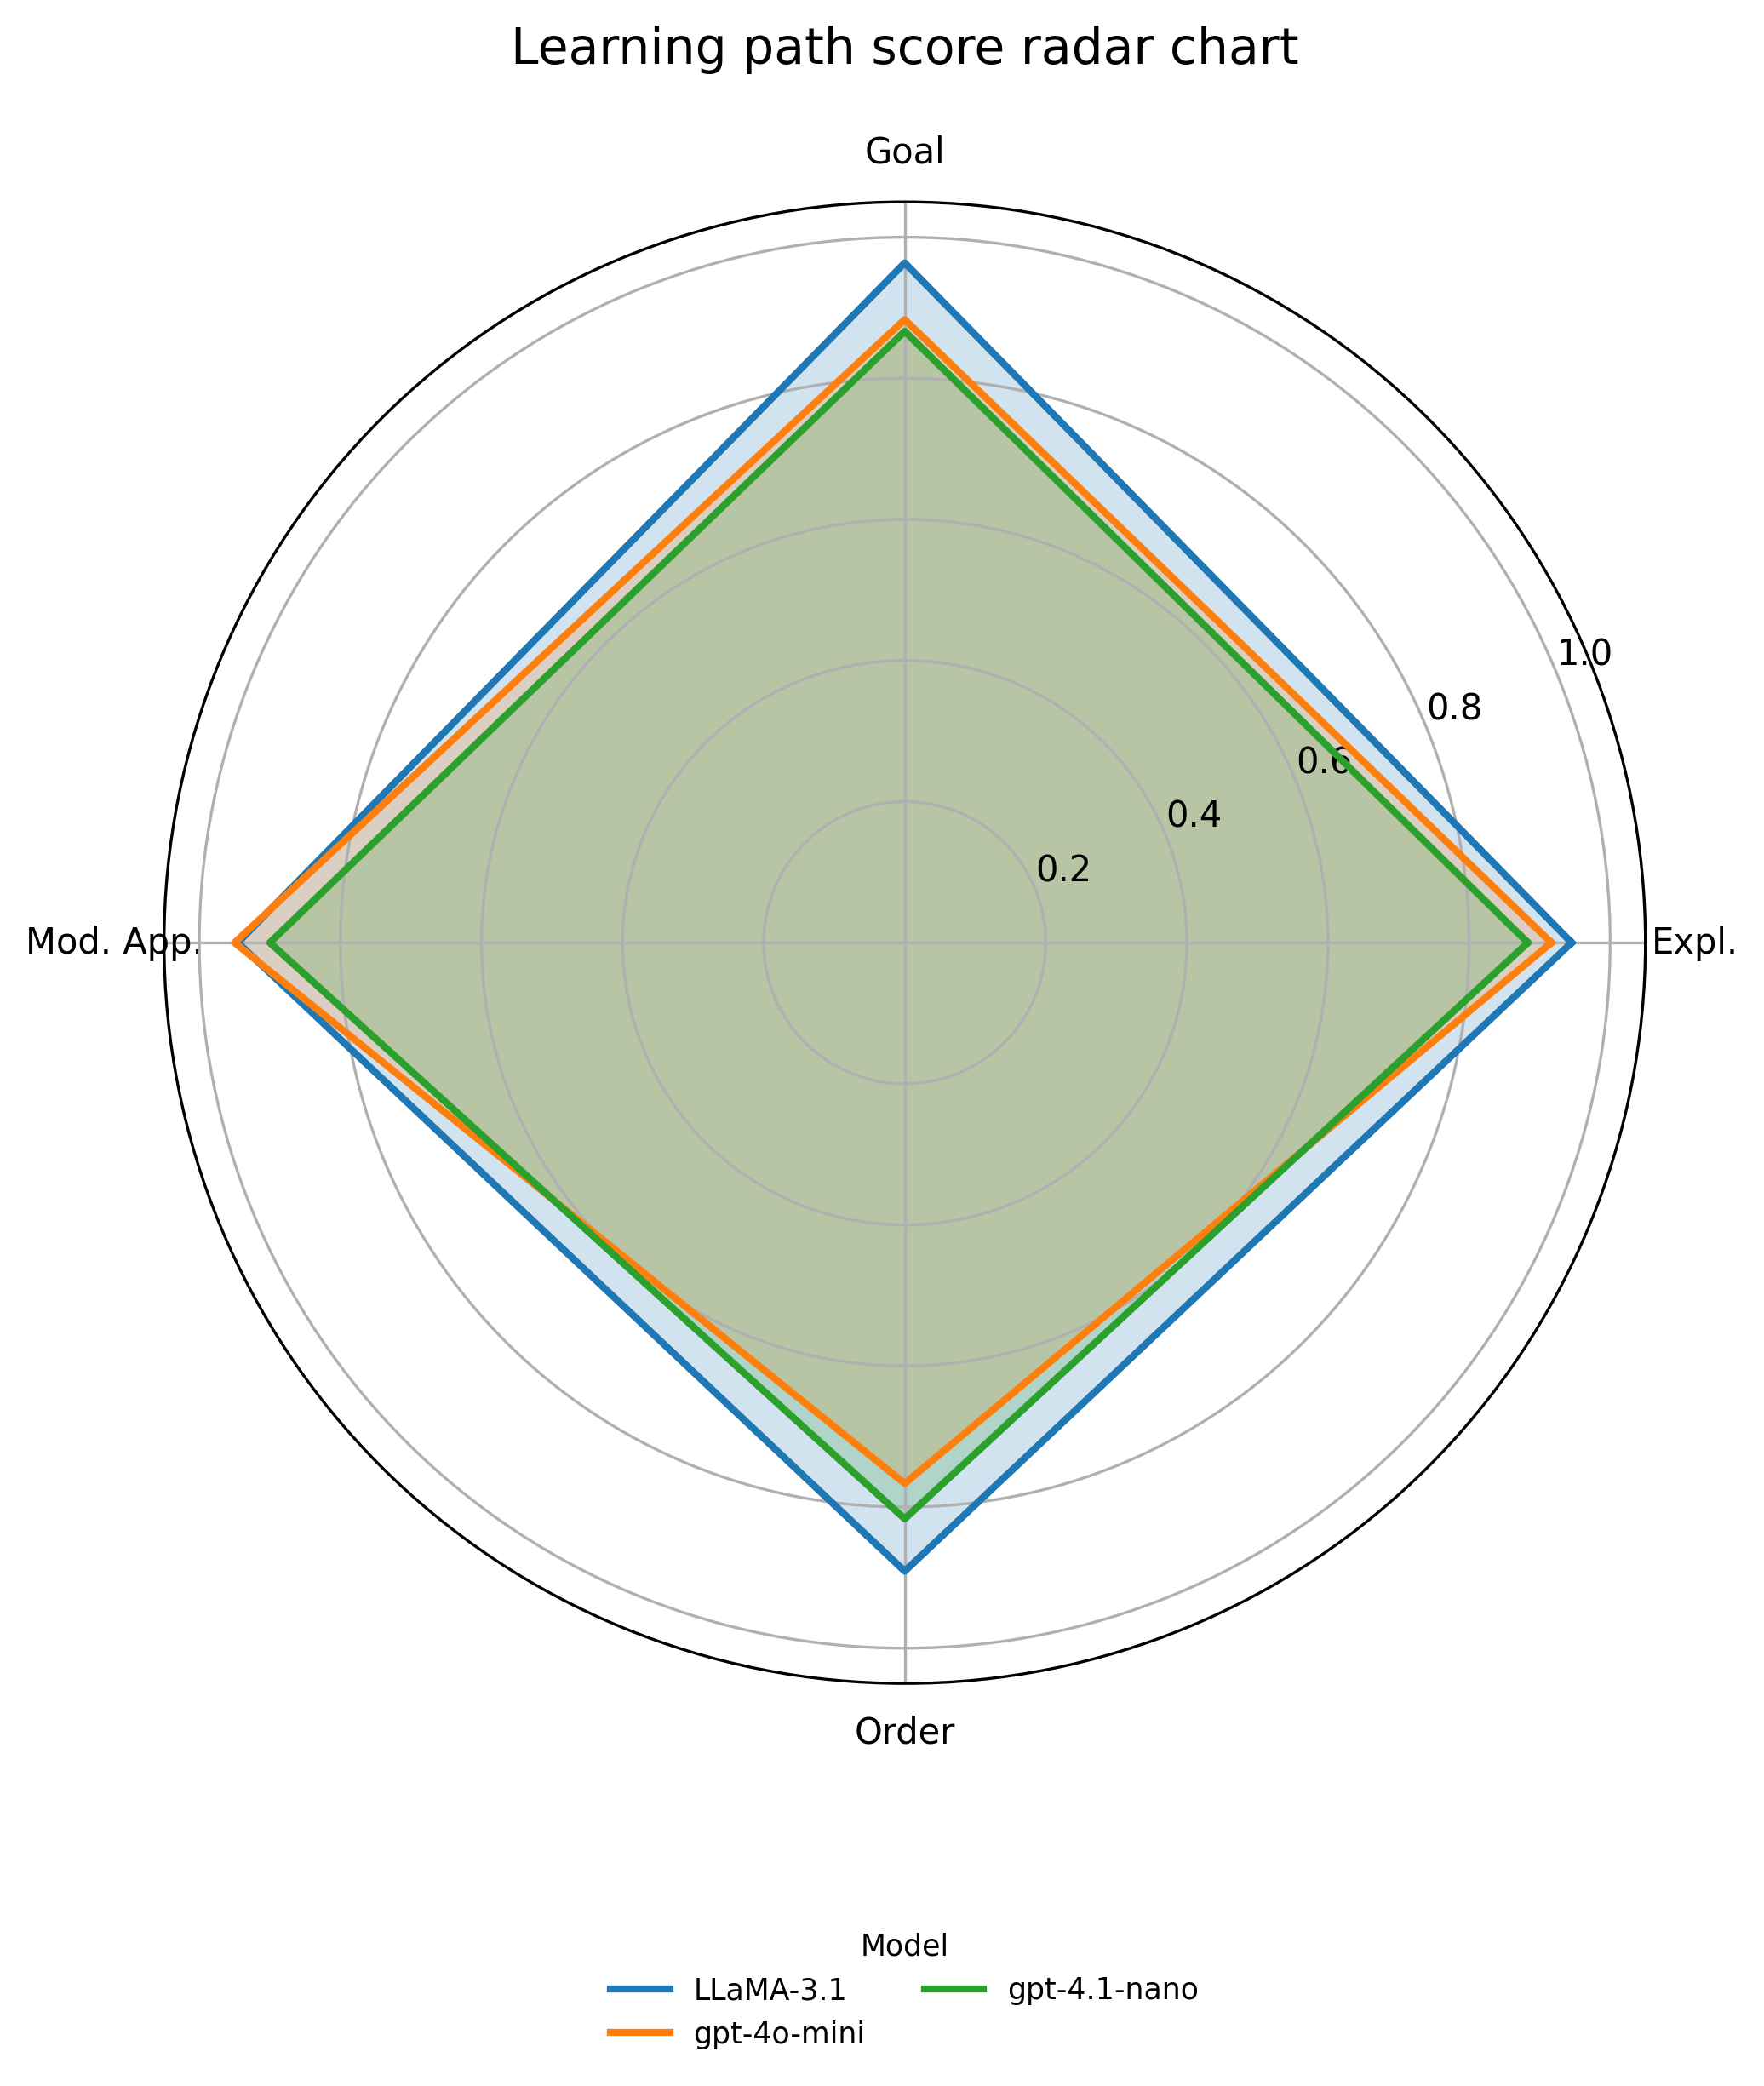
\includegraphics[width=0.6\textwidth]{images/lp_eval_radar_chart.png}
    \caption{Radar chart tổng hợp kết quả đánh giá lộ trình học đề xuất khi chạy đánh giá LLM-as-a-judge ứng với từng model}
\end{figure}

Dựa vào kết quả có được, sau đây là một số nhận xét sơ bộ:
\begin{itemize}
    \item Tiêu chí \textbf{Explanation Quality} đạt điểm trung bình cao nhất (0.917 theo gpt-4o-mini hay 0.883 theo gpt-4.1-nano), cho thấy phần lớn các bài học trong lộ trình đều có phần giải thích rõ ràng, dễ hiểu và phù hợp với nội dung.

    \item Về tiêu chí \textbf{Module Appropriateness}, hệ thống cũng ghi nhận mức đánh giá tích cực (lên đến 0.95), cho thấy các module học tập được lựa chọn và tạo sinh phù hợp với từng bài học và mục tiêu tổng thể, không bị lệch pha hay dư thừa nội dung.

    \item Tiêu chí \textbf{Goal Alignment} có điểm số ổn định (khoảng 0.88), phản ánh rằng lộ trình học tập nhìn chung bám sát mục tiêu đầu vào mà người học đã đặt ra.

    \item Tuy nhiên, ở tiêu chí \textbf{Ordering Logic}, điểm số trung bình thấp hơn đáng kể (0.767 theo gpt-4o-mini, 0.817 theo gpt-4.1-nano). Điều này cho thấy vẫn còn tồn tại một số vấn đề về thứ tự sắp xếp các bài học – ví dụ như thiếu tính tuyến tính, sắp xếp không tối ưu về mặt xây dựng nền tảng kiến thức.
\end{itemize}

\section{Đánh giá testcases được sinh ra bởi hệ thống}
\subsection{Phương pháp đánh giá}
Trong bối cảnh đánh giá chất lượng test case được sinh tự động bởi LLM nói riêng cũng như chất lượng của một bộ testcases nói chung, có nhiều metrics khác nhau có thể được xem xét, bao gồm:
\begin{itemize}
    \item Tính đa dạng (Diversity) đo mức độ khác biệt giữa các test case trong một bộ dữ liệu.
    \item Độ phủ (Coverage) đo xem test case có bao phủ đủ các nhánh logic, điều kiện biên, hoặc tập input không.
    \item Mutation Score là tỉ lệ mutant (phiên bản lời giải bị chỉnh sửa nhỏ để cố tình tạo lỗi) bị phát hiện bởi test case. Chỉ số này phản ánh khả năng của test case trong việc phân biệt giữa lời giải đúng và lời giải sai — tức là đo mức độ “sắc bén” của test case trong kiểm thử.

\end{itemize}

Tuy nhiên, trong phạm vi đánh giá sơ bộ này, nhóm lựa chọn một metric đơn giản nhưng có giá trị thực tiễn là: \textbf{tỉ lệ test case chạy đúng (pass)} khi thực thi với một lời giải đã được kiểm chứng là chính xác với các lý do như sau:
\begin{itemize}
    \item Đây là bước kiểm tra cơ bản và thiết yếu, nếu test case không chạy được hoặc gây lỗi, các đánh giá khác sẽ không còn ý nghĩa.
    \item Dễ triển khai và so sánh giữa các mô hình sinh test case khác nhau.
    \item Phản ánh gián tiếp khả năng hiểu đề và sinh đầu vào hợp lệ của mô hình.
\end{itemize}

Phép đánh giá được thực hiện bằng cách chạy từng test case trên một lời giải mẫu được xác nhận là đúng, sử dụng môi trường thực thi tự động (Judge0). Các kết quả như “Pass”, “Fail”, “Runtime Error” được ghi nhận và tổng hợp theo từng mô hình LLM để phân tích định lượng.

\subsection{Cài đặt}
Sau đây là cấu hình cho phần đánh giá:
\begin{itemize}
    \item Các mô hình được sử dụng: \emph{gpt-4o-mini}, \emph{gpt-4.1-nano}, \emph{gemini-2.0-flash}.
    \item Bài tập lập trình: 12 bài tập lập trình được lựa chọn ngẫu nhiên trên các trang: \url{leetcode.com}, \url{hackerrank.com},... và lời giải được kiểm chứng. Về dữ liệum, người đọc có thể xem chi tiết ở \href{https://github.com/dpnam2112/codemate-backend/blob/main/evaluation/data/leetcode_problems/leetcode.json}{đây}(\footnote{\url{https://github.com/dpnam2112/codemate-backend/blob/main/evaluation/data/leetcode_problems/leetcode.json}})
    \item Sử dụng mỗi mô hình để tạo sinh testcases cho mỗi bài tập, trung bình với mỗi bài sẽ có từ 8 tới 14 testcases (Tùy thuộc vào mô hình cũng như giới hạn tính toán được áp đặt bởi nhà cung cấp dịch vụ để gọi mô hình: OpenAI, TogetherAI, Google VertexAI).

\end{itemize}

\subsection{Kết quả đánh giá và nhận xét}

\begin{table}[H]
\centering
\begin{tabular}{lrrrr}
\toprule
\textbf{LLM Model} & \textbf{Total} & \textbf{Pass} & \textbf{Fail} & \textbf{Runtime Error} \\
\midrule
gpt-4o-mini            & 147 & 79.6\% & 19.0\% & 1.4\%  \\
gpt-4.1-nano           & 125 & 84.8\% & 13.6\% & 1.6\%  \\
gemini-2.0-flash-lite  & 161 & 77.0\% & 16.8\% & 6.2\% \\
llama-3.3-70B-Instruct & 74  & 51.4\% & 31.1\% & 17.6\% \\
\bottomrule
\end{tabular}
\caption{Tổng quan kết quả thực thi test case sinh bởi LLM}
\vspace{0.5em}
\noindent
\textit{\textbf{Chú thích cột:}} 
\textbf{Total} là tổng số test case được sinh ra và đánh giá. 
\textbf{Pass} là tỉ lệ test case cho ra kết quả đúng khi chạy với lời giải chính xác. 
\textbf{Fail} là test case chạy được nhưng cho kết quả sai. 
\textbf{Runtime Error} là test case gây lỗi khi thực thi (ví dụ chia cho 0, lỗi kiểu dữ liệu,...).
\end{table}

\emph{Nhận xét: }

Tổng quan kết quả đánh giá cho thấy các mô hình LLM có khả năng sinh test case ở mức khá, với tỷ lệ Pass trung bình từ 75\% trở lên đối với các mô hình của OpenAI và Gemini. Trong đó, mô hình \textbf{gpt-4.1-nano} đạt kết quả cao nhất với 84.8\% test case được đánh giá là đúng (Pass), cho thấy khả năng hiểu bài toán và sinh dữ liệu kiểm thử hợp lý. Mô hình \textbf{gpt-4o-mini} theo sau với tỷ lệ 79.6\%, tuy nhiên tỷ lệ test case sai (Fail) cao hơn, cho thấy chưa bao phủ đủ các trường hợp đặc biệt (edge cases).

Đáng chú ý, mô hình \textbf{gemini-2.0-flash-lite} có số lượng Runtime Error cao hơn (6.2\%), phản ánh khả năng sinh input chưa ổn định hoặc dễ gây lỗi khi thực thi. Mô hình \textbf{llama-3.3-70B-Instruct} có kết quả thấp nhất với chỉ 51.4\% Pass và tỷ lệ Runtime Error lên đến 17.6\%, cho thấy khó khăn trong việc sinh ra các test case chính xác và phù hợp định dạng.

Các nguyên nhân chính dẫn đến lỗi test case gồm:
\begin{itemize}
    \item \textbf{Hạn chế về khả năng xử lý số liệu:}: LLM không được thiết kế để thực hiện tính toán, dẫn đến việc sinh output sai hoặc không nhất quán.
    \item \textbf{Sai định dạng input/output:} Một số testcase bị lỗi do định dạng không đúng với yêu cầu, ví dụ như thiếu dòng newline, thiếu ký tự phân cách hoặc kiểu dữ liệu không khớp.
\end{itemize}
\subsubsection{Hướng phát triển và cải thiện cho phần tạo sinh testcases}

Kết quả đánh giá cho thấy các mô hình LLM hiện tại tuy có khả năng sinh test case hợp lệ ở mức khá, nhưng vẫn còn tồn tại một số nhược điểm như sai định dạng, thiếu bao phủ edge cases, và sinh ra dữ liệu không ổn định gây lỗi khi thực thi. Để khắc phục và cải thiện chất lượng đầu ra, một số hướng phát triển có thể được xem xét như sau:

\begin{itemize}
    \item Fine-tune mô hình: Việc huấn luyện lại mô hình (fine-tune) trên tập dữ liệu chứa các bài toán lập trình và test case đúng chuẩn có thể giúp mô hình học được cấu trúc và định dạng đầu ra mong muốn, từ đó giảm thiểu các lỗi định dạng hoặc logic phổ biến.

    \item Tích hợp function calling: Việc sử dụng cơ chế function calling (ví dụ như OpenAI Tools API hoặc ReAct-style prompting) cho phép mô hình gọi các hàm kiểm tra định dạng, phân tích cú pháp hoặc validate input/output trong quá trình sinh test case. Điều này giúp phát hiện và loại bỏ các test case không hợp lệ ngay từ bước sinh.
\end{itemize}
